\emph{
    Tome el límite conforme $p\to 0$ para mostrar que la variable aleatoria 
    \begin{align}
        M=-\min_{n\geq 0}S_n
    \end{align}
    tiene una distribuci\'on geom\'etrica de par\'ametro $1-e^{-f(1)}$. Interprete esto cuando $f(1)=0$.
}

Cuando hablamos de $C_p$, sólo nos interesa su distribución.\par\null

Así que para ejemplificar cómo se comporta una suceción de geométricas con sus parámetros tendien a $0$,
mientras conservemos a $C_p$ con distribución geométrica, somos libres de elegir de que manera se comportan.\par\null

Definamos $C_p : [0,1] \rightarrow \N$ (donde en $[0,1]$ usamos la medida de Lebesgue) de la siguiente manera:

\begin{align}
    C_{p}(x) = 
        \begin{cases}
            1       & \mbox{if } x \in [0, p)                                                                               \\
            2       & \mbox{if } x \in [p, p + (1-p)p)                                                                      \\
            \vdots  &                                                                                                       \\
            n       & \mbox{if } x \in \bigg[\sum_{i = 1}^{n - 1} (1 - p)^{i - 1}p , \sum_{i = 1}^n (1-p)^{i-1}p \bigg)     \\
            \vdots  &                                               
        \end{cases}
\end{align}

Claramente, $C_p$ definida de esta manera tiene distribución de una geométrica de parámetro $p$ (Porque no le dejamos de otra).\par\null

Ahora podemos ver con más claridad que 

\begin{align}
    \mw(C_p > n) = 1 - \sum_{i = 1}^n (1-p)^{i-1}p
\end{align}

Analicemos la derivada del término $(1-p)^{i}p$ ($i$ fija) con respecto a $p$. Su derivada es $(1-p)^i - p i (1-p)^{i-1}$.
Evaluando en $0$ tenemos \\
$(1-0)^i - 0 i (1-0)^{i-1} = 1 > 0$. Es decir que cerca de $0$, cada uno de los términos de este tipo, es 
estrictamente creciente.\par\null

Es decir, que si $p$ se va acercando hacia 0, cada uno de estos términos, decrece.\par\null

A continuación una gráfica de cómo se comporta $1 - \sum_{i = 1}^{100} (1-p)^{i-1}p$ conforme variamos $p$.
(Se incluye el script de R que se implementó para realizar esta gráfica, junto con algunas otras gráficas para
distintos valores de $n$).\par\null

\begin{center}
    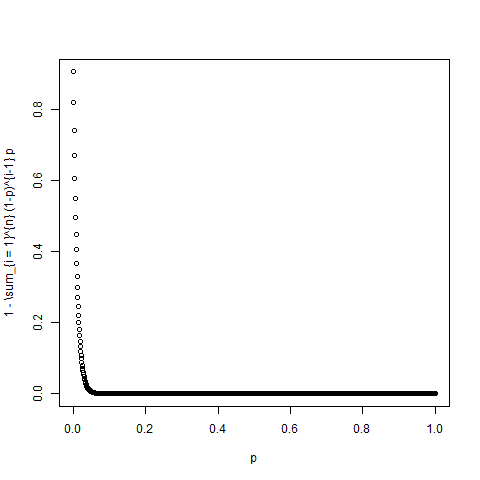
\includegraphics[width=6cm]{tarea2/problema2_1/graficas_inciso2_1_4/probabilidadDeQueC_pSupere100.png}
\end{center}\par\null

Con todo esto dicho, podemos garantizar que $C_p$ diverge a $\infty$ en distribución. Pues para todo rango $[m, n]$ con $m<n,\in \N$
$\mw(C_p \in [m, n]) \rightarrow 0$. \par\null

Entonces 
\begin{align}
    - \min_{n \leq C_p} \rightarrow - \min_{n \leq \infty} S_n = \min_{n \geq 0} S_n = M
\end{align}\par\null

Ahora recordemos que $g$ era una función continua y que $g>0$. Por lo tanto $1/g$ es una función continua,
con inverso derecho $f$ en $(0, 1)$. Es decir

Por lo tanto
\begin{align}
    \mw(M = n)  &=  \lim_{p \rightarrow 0} \mw(M_p = n)                         \\
                &=  \lim_{p \rightarrow 0} e^{-n f(1-p)}(1-e^{- f(1-p)})        \\
                &=   e^{-n f(1)}(1-e^{- f(1)}) \label{problema2_1:distribucion_de_M}
\end{align}

Lo cual corresponde a la distribución de una geométrica de parámetro $1-e^{- f(1)}$.\par\null

El caso donde $f(1^-) = 0$, implica que $\lim_{p\rightarrow0} (1-e^{- f(1-p)}) = 0$. El cual es complétamente
análogo al caso anterior donde considerábamos $p \rightarrow 0$ en geométricas de parámetro $p$.\par\null

Donde, habíamos dejado claro que conforme el parámetro disminuía hacia 0, las distribuciones de las geométricas divergía 
a la de $\infty$ y que por lo tanto la probabilidad de que nuestras geométricas tomaran cierto 
valor $n$ disminuía hacia $0$ conforme el parámetro tendía a $0$.\par\null

Incluso para este caso, la ecuación \eqref{problema2_1:distribucion_de_M} es válida según nuestro análisis, pues

\begin{align}
\mw(M = n)  &=  \lim_{p \rightarrow 0} \mw(M_p = n)                         \\
                &=  \lim_{p \rightarrow 0} e^{-n f(1-p)}(1-e^{- f(1-p)})    \\
                &=  e^{-n 0}(1-e^{- 0})                                     \\
                &=  1(1-1)                                                  \\
                &=  0.
\end{align}

Y esto, para toda $n \in \N$, justo como nuestro análisis de las distribuciones geométricas
nos dijo.